\documentclass[12pt,a4paper]{article}

\usepackage{pdfpages}
\usepackage{indentfirst}
\usepackage{graphicx}
\usepackage{amsmath}
\usepackage{epstopdf}
\usepackage{url}
\usepackage{tikz}
\usepackage{hyperref}

\begin{document}

\title{Traffic Stop Bias Paper}
\author{David Ford}
\maketitle


\section{Abstract:}

In recent years, concerns and discussions surrounding discriminatory treatment of minority citizens by the police have grown. Most notably the ``Black Lives Matter" (BLM) movement has placed a spotlight on black deaths. As BLM grew, activists made specific efforts to humanize the victims of systemic racism - and ``Say Their Name" (STN) was born. In this paper, I analyze police interactions by exploring changes in traffic stop behaviors using a large and novel dataset combination of traffic stops and fatal police encounters, supplemented with internet search data to infer death-event scrutiny levels. I find that policing efforts decrease following low-scrutiny events, but contraband-finding rates remain stable; findings consistent with police officers reducing proactivity following a fatal mistake - when they are not being watched closely. \\

\footnote{DRAFT - DO NOT CIRCULATE} \\

%%%%%%%%%%%%%%%%%%%%%%%%%%%%%%%%%%%%%%%%%%%%%%%%%%%%%%%%%%%%%%%%%%%%%%%%%%%%%%%%%%%%%%%%%%%%%%%%%%%%

\section{Introduction:} 

After the 2012 death of Trayvon Martin, a 17 year-old boy who was shot to death by one of his neighbors (George Zimmerman), protests broke out nationwide. Following this, in July 2013 Zimmerman was acquitted for Trayvon's death, which sparked further outrage and led to the coining of Black Lives Matter (BLM), and the beginning of a movement as many felt that the justice system had failed both to protect Trayvon and to punish his killer. \\

In the following year the movement grew and evolved, and the phrase ``Say Her Name" was coined, with the specific intent of humanizing female victims of systemic racism, quickly transforming into the wider ``Say Their Name" variation more commonly seen today. The basic premise is simple: these were people, they mattered, and their deaths are not simple blips in the system to be glossed-over. By making efforts to use their names, the attention might shift from ``unarmed black subject killed by police last week" to ``Eric Garner asphyxiated by police with prohibited chokehold during arrest for selling loose cigarettes". \\ 

BLM has since become the rallying cry of many protestors throughout the nation - becoming one of the more popular internet hashtags and drawing a lot of attention to a number of deaths that may have otherwise gone unnoticed by the general public; Michael Brown, Alton Sterling, Philando Castile, Breonna Taylor, and George Floyd to name a few. \\

By resulting in a death, these are significant events, and with each successive death the possibility of dying at the hands of the police becomes more salient and concerning for many Americans. In fact, deaths by police account for 5\% of all homicides int he US (Ang \& Tebes 2023). As such, these deaths deserve attention, particularly in the context of further police interactions. To accomplish this, I will be using the open source Fatal Encounters (FE) dataset which tracks officer-involved subject-deaths in the US going back to 2000. \\

In order to scrutinize the most significant type of police encounter, this study combines subject-death data with data on the most frequent type of police interaction; traffic stops. At 50k/day, traffic stops are by far the most frequent police interaction. To accomplish this, I use the Stanford Open Policing Project (SOPP) data, which is the largest available dataset on US traffic stops and was created by a team of researchers making data requests to numerous departments across the nation. \\

Merging the SOPP and FE datasets allows me to closely consider the timing of traffic stops and searches surrounding these momentous deaths and to look closely for observed changes in behavior. Specifically, I consider the probability of a stopped driver being black, the search rate for black drivers, and the search success rate for black stops, i.e. the ``hit rate". \\

Theoretically, a police officer receives a set of unobserved signals during a traffic stop, and they use this information to determine whether or not to search a vehicle. Of course they consider day of week, stop location, observed driving behavior, but they also observe a variety of driver characteristics such as perceived race and age and many intangible characteristics of the driver and their passengers, such as nervousness and general demeanor. After observing this set of signals, many of which are not recorded, the officer considers the likelihood of that driver carrying contraband and decides whether or not to carry out a search of the vehicle, which then may or may not result in a hit. \\

In the wake of an officer-involved subject-death, the law enforcement agency and its officers receive a pronounced level of scrutiny, sometimes on the national stage for the more-scrutinized subject-deaths. With this, the perceived cost of stopping or searching a car may grow as officers are forced to consider the increased negative attention they are gaining in the public eye and the risk of becoming a star in the next viral video admonishing the police. \\

Additionally, and separately from this increased cost consideration, it may be that police officers feel less valued in their efforts to combat crime when they see widespread protests against them, which may lead to a de-policing effect as police officers receive fewer intangible rewards such as public gratitude and therefore reduce effort levels (Powell 2022). Either of these effects would be consistent with my finding that police efforts decrease following a lethal mistake. \\

As a result of the above effects, police officers may become less willing to stop or search \emph{marginally suspicious} cars. This effect should be the particularly-pronounced in stops/searches of black drivers, the focus of the BLM movement. With these considerations, theory might expect these effects to encourage fewer stops, fewer searches, and a higher hit rate as officers are less likely to search marginally-suspicious drivers, preferring only to search those drivers when they have a high expectation of success. However, my findings point to a different conclusion - that policing efforts decrease, but once a stop has been made, what follows is ``business as usual". \\

To contrast this officer-side increase in scrutiny, the drivers on the road may behave differently. As a driver, particularly as a black driver, in the aftermath of seeing news about a potentially-unjustified black subject death, the perceived-risk of a police interaction may become more salient. This may lead to more careful driving behavior, and a decrease in the likelihood of carrying contraband for the marginal driver, particularly the marginal black driver. Either of these two effects should lead to lower black stop probabilities and lower search rates, and perhaps a lower hit rate as drivers are less willing to risk escalating a police encounter. While I do find that black stops decrease, they do so disproportionately to the decrease in non-black stops, a finding. \\

In order to explore these potentially-conflicting effects in detail, I analyze traffic stop data in two main ways. First, I consider the full set of 150 focal deaths of an \textit{unarmed black subjects} that are \textit{shot, bludgeoned, or asphyxiated} to see if the death itself leads to any changes in observable traffic stop behaviors, and then I use Google Trends search data to infer which deaths were scrutinized more heavily based on Google Trends search patterns for the deceased's names. \\

%%%%%%%%%%%%%%%%%%%%%%%%%%%%%%%%%%%%%%%%%%%%%%%%%%%%%%%%%%%%%%%%%%%%%%%%%%%%%%%%%%%%%%%%%%%%%%%%%%%%

\section{Literature Review:}
%%%% On minority drivers: %%%
Looking at the existing body of research, it has been shown that minorities drivers are treated differently than white drivers. By looking at 2015-2016 Trump campaign rallies, it has been shown that police officers are more likely to stop black drivers for up to 60 days following a Trump campaign in the county (Grosjean, Masera \& Yousef, 2022). Minority drivers are also given fewer discretionary ``discounts" in their speeding tickets (Goncalves \& Mello, 2021). Black drivers cars are more likely to be searched (Knowles, Persico \& Todd, 2001). Police appear to have a lower inferred threshold for search black and hispanic drivers (Pierson et al, 2020). It has even been shown that the language used by officers when talking to black drivers is less respectful, less formal, and less impartial (Voigt et al 2017). Perhaps as a result of these lopsided search practices, it has been shown that black drivers may adjust their driving patterns by driving more carefully in the daylight, when they believe themselves more likely to be noticed by the police (Kalinowski, Ross \& Ross, 2021). \\

%%% On minority citizens: %%%
Minority citizens have been shown to receive disfavorable treatment off the road as well. White Law Enforcement Officers (LEOs) are more likely to use force in minority neighborhoods compared to black LEOs (Hoekstra \& Sloan, 2022). Stereotypical minority clothing and neighborhoods have been experimentally shown to increase the likelihood of being shot in psychological studies (Khan \& Davies, 2017). In meta analysis studies, relative to white targets armed black targets are more likely to be shot, unarmed black targets are slower to \textit{not} be shot, and black targets have a lower overall threshold for being shot (Mekawi \& Bresin, 2015). \\

%%% Problems with estimating: %%%
Many attempts have been made in the past to evaluate traffic stop bias. One recurring issue however is that the number of black drivers on the road is unobserved, as such the stop rate is difficult to define in a compelling way. Various methods have been suggested to avoid measurement errors, such as using ``not-at-fault" traffic crashes as an ``as good as random" estimate for the share of black drivers on the road (Alpert, Smith \& Dunham, 2004). Another novel approach using visibility and daylight conditions has been suggested as well, with the idea being that police officers are less able to determine that a driver is black when it is dark outside, allowing daylight savings time changes to serve as a proxy for police officer visibility (Grogger \& Ridgeway, 2006), although there are some concerns that streetlights and other light sources could dilute the seemingly-clear relationship between daylight and visibility that is difficult to address (Horrace \& Rohlin, 2016). \\

%%% Existing Estimation Strategies: %%%
It has long been suggested that post-decision outcomes, such as hit rates, might be used to evaluate potential bias in vehicle search decisions (Becker 1957, 1993). However, more recent research has suggested that this practice might suffer from infra-marginality if the unobserved contraband-carrying distributions differ along race, with a suggested \textit{extremely} computationally-expensive threshold test using Bayesian latent variable modelling to repeatedly sample and estimate contraband-carrying rates as well as search-decision thresholds simultanseously (Simoiu, Corbett-Davies \& Goel, 2017). More recently, a less-demanding ``discrimnant distributions" workaround has been put forth by many of the same authors (Pierson, Corbett-Davies, \& Goel, 2018). Lastly, officer-race might be useful to mitigate concerns as discriminatory search practices, if they are motivated by statistical discrimination, should be constant across officer race - a testable feature of this dataset (Antonovics \& Knight, 2009). \\

%%% The other side: %%%
As for the policing side of things, officer sentiments and public scrutiny have been shown to influence policing decisions. Following the death of Michael Brown in Ferguson, MO, a de-policing effect is found where officer-initiated actions such as traffic stops decrease as a result of negative public scrutiny (Powell, 2022). Additionally, in somewhat of a ``mirror" to this study, officer deaths have been shown to increase saliency of workplace risks for police officers, leading to reductions in low-level arrests (Cho, Goncales \& Weisburst, 2023). \\

%%% Defending my choices: %%%
In a meta analysis of nearly 1,200 peer-reviewed articles across the exact years used in this study, citizen weapon possession was shown to be the most consistent predictor of police usage of deadly force (Mora, Terrill \& Foster, 2022), as a result only unarmed deaths are considered in this study. On the choice of using the open-source Fatal Encounters dataset, it has been shown to be preferable to various government sources of death-by-police measurements (Finch et al, 2019), and compared to other open-source datasets it appears to be the most reliable (Renner, 2018). \\

%%% Possible solutions: %%%
As far as strategies to reduce these violent encounters go, Department of Justice (DOJ) consent decrees have been shown as ineffective (Goh, 2020), although mental health treatment center availability has been shown to reduce assaults committed against police officers (Deza, Lu, MacLean \& Ortega, 2023). Lastly, it has been shown that proximity to a fatal police event increases civic engagement by way of voting and voter registration, particularly for black and hispanic citizens following unarmed subject-deaths which could be an interesting avenue for future research (Ang \& Tebes 2023). \\

%%%%%%%%%%%%%%%%%%%%%%%%%%%%%%%%%%%%%%%%%%%%%%%%%%%%%%%%%%%%%%%%%%%%%%%%%%%%%%%%%%%%%%%%%%%%%%%%%%%%

\section{Data:}

For this paper, I use three primary data sources. The Stanford Open Policing Project (SOPP), Fatal Encounters (FE), and Google Trends (Trends), which I break down in further detail below. \\


\subsection{The Stanford Open Policing Project: Traffic Stop Data:}

The SOPP data consists of traffic stop information for 88 different locales throughout the continental US which were acquired via FOIA requests by a team of Stanford researchers which I then cleaned and appended together. Figure 1 depicts the SOPP data coverage. \\

\begin{figure}
	\begin{center}
		\includegraphics[width=6.0in]{stop_data_map.eps}
		\caption{In the above figure, dark gray states correspond to those states with both state patrol + full local jurisdictional data such as Illinois, light gray to those with only state patrol data, white to those with no statewide data, and the red dots correpond to municipal data such as that of LA, with larger red dots indicating a larger number of stop observations.}
		\label{sopp_map}
	\end{center}
\end{figure}

To clean the data, first, I de-duplicated the four overlapping-jurisdictions in the data, e.g. Chicago, Illinois vs Statewide-Illinois which had unwanted overlapping observations. An issue arose with unreliable department-naming practices in the SOPP dataset, forcing me to rename departments for consistency and to allow a later merge with the FE dataset. I manually looked for the actual name for each department changed them to align with FE conventions, e.g. ``LMPD" and ``Louisville Metro PD" were changed to align with ``Louisville Metro Police Department" from the FE dataset. \\

Because this analysis relies heavily on event-timing, I was forced to drop a number of departments that only reported stop data at the monthly or annual level. If a department always reported stops on the same day of each month, these were identified as ``monthly reporters" and dropped, similarly for ``annual reporting" departments which always reported stops in the same month. With demanding event-timings, these departments were not usable. As my analysis also relies on the race of the stopped driver, any departments which \emph{never} record a black stop have been removed as well. \\

After this, following a few conventions from existing literature, I went on to drop pedestrian stops from the analysis, as I am focusing on traffic stop behaviors. I also dropped ``consent" searches as these are inherently different and the direct permission to search a vehicle avoids the officer's search decision almost entirely. Lastly I drop ``plain view" searches as these searches in theory should all have a 100\% success rate which would bias my results. For my main analysis, I also drop statewide-departments, i.e. California and Texas Highway Patrols, as I believe these departments with their incredibly-wide coverage areas are inherently different from more localized departments. This restriction is removed as a robustness check, which is left in the forthcoming online appendix. \\

Within the resulting cleaned SOPP data, I have traffic stop observations along with information such as which department makes the stop, which day the stop occurred on, whether a search was conducted, and whether contraband was found. In the near future, I intend to also use officer race data to explore whether behavior patterns vary across race, which would serve as evidence against pure statistical disctimination, as mentioned above. \\


\subsection{Fatal Encounters: Event Timing Data:}

Beginning in 2012, the FE began collecting information on police-killings in the US with a team of volunteer researchers via FOIA requests, scouring newspaper articles, and crowdsourced submissions which were then checked and added to the database. Their stated goal is to construct an ``impartial, comprehensive, searchable national database of people killed during interactions with the police'', and they have back-collected data going back to 2000. As it stands, this appears to be the most-reliable source of officer-involved-death information in the United States, surpassing even the official government reckonings which have been shown to oftentimes contain errors or omit deaths entirely. \\

Starting from their basic data download of nearly 31,500 deaths, I chose to use a limited subsample of these fatal encounters to capture a specific type of death deemed most-relevant to my analysis. First, I want to capture the deaths where I have information about subject-armedness, which limits me to the 2011-2018 period because subject-armedness is not tracked for deaths before 2011, which reduces my potential events to 17,149, out of which 6,128 subjects were listed as unarmed. Next, I am specifically interested in black deaths as per my research question, of which there remain 1,814. After this I consider only shooting/bludgeoning/asphyxiation deaths as these are the deaths where direct and potentially-lethal force was used, as opposed to deaths with less-direct lethal intentionality, e.g. car crashes, drownings, lethal falls, and less-than-lethal options such as tasers or pepper spray, which leaves me with a maximum of 614 events which could be matched with traffic stop data. \\

After merging the SOPP+FE datasets together, I was left with 152 matched-focal-events, meaning, 152 unarmed black subjects who were shot, bludgeoned, or asphyxiated by the police between 2011 and 2018. Due to concerns with observations that were attributed to multiple involved-departments, concerns with exact event timing identification, and concerns with the specific nature of these deaths, I manually looked into each of the 152 deaths. In doing so, I was able to pinpoint precisely which department caused the death in all of my multi-department events, I was able to confirm and fix event timings, and I was able to verify the nature of each death and remove a few that were not warranted under the goals of my study, e.g. murder-suicides, and a few hostage-executions. \\

What remained after this dropping process was a reliable set of deaths and event dates to be analyzed. All told, I have 60 usable death-events for my analysis, 29 of which are classified as high-scrutiny events. \\

%%% DESCRIPTIVE STATISTICS FIGURE %%%
\begin{figure}
	\begin{center}
		\includegraphics[width=5.5in]{desc_stats}
		\caption{In the above graph, the data is split up into control vs treatment, and black vs non-black. The right column shows row-totals for the number of stops, searches, and hits, with the respective percentages depicting the share of the total that belongs to each of the four split groups. Additionally, the raw search rates and hit rates are split up by category and shown.}
		\label{desc_stats}
	\end{center}
\end{figure}

\subsection{Google Trends: Public Scrutiny Data:}
In order to assess whether public attention influences traffic stop behaviors, a proxy was required to infer scrutiny levels for each subject-death. Following naturally from the ``Say Their Names" movement that began and grew throughout much of my sample, I manually-pulled internet search relative-volumes using Google Trends. As the website only gives relative-volumes, this required a benchmark event to scale all events to allow comparisons. I chose my most-searched name and its corresponding department - Michael Brown and the Ferguson Police Department to determine two sets of relative-search-frequencies. \\

As a robustness-check against this method of scrutiny-inference, I have also manually curated a list of ``publicized deaths" based on a suitably-named and directly-relevant ``Say Their Names" online exhibit from the Stanford Library, under which the results remain largely similar. \\

%%%%%%%%%%%%%%%%%%%%%%%%%%%%%%%%%%%%%%%%%%%%%%%%%%%%%%%%%%%%%%%%%%%%%%%%%%%%%%%%%%%%%%%%%%%%%%%%%%%%

\section{Methodology \& Results:}

For the purposes of this paper, a department is considered treated if one of its officers is observed fatally shooting, bludgeoning, or asphyxiating an unarmed black subject between 2011 and 2018. Each traffic stop is then assigned an ``event time" based on the number of days to the nearest event. As a result, any department with multiple observed-events has each of its traffic stop dates matched to the \textit{nearest} event date, as demonstrated in Figure 3. \\

\begin{figure}
	\begin{center}
		\noindent \underline{-Single-Event Departments} \\
		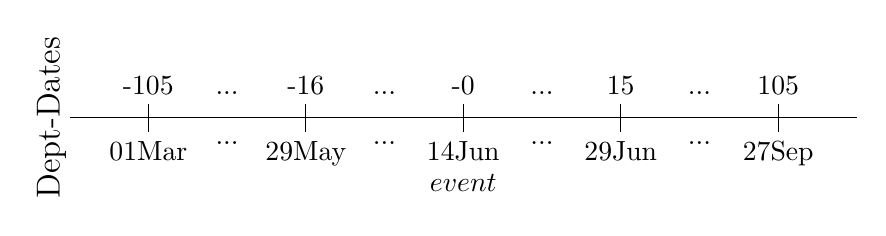
\begin{tikzpicture}
			\draw (0,0) -- (10,0);
			\foreach \x in {1, 3, 5, 7, 9}
			\draw (\x, 5pt) -- (\x, -5pt);
			\draw (1,0) node[below=5pt] {01Mar} node[above=5pt] {-105};
			\draw (3,0) node[below=5pt] {29May} node[above=5pt] {-16};
			\draw (5,0) node[below=5pt] {14Jun} node[above=5pt] {-0};
			\draw (5,0) node[below=17pt] {$event$};
			\draw (7,0) node[below=5pt] {29Jun} node[above=5pt] {15};
			\draw (9,0) node[below=5pt] {27Sep} node[above=5pt] {105};
			\foreach \y in {2, 4, 6, 8}
			\draw (\y,0) node[below=5pt] {...} node[above=5pt] {...};
			\path (0,0) -- (10,0) node[rotate=90,midway,sloped,above=140] {\large Dept-Dates};
		\end{tikzpicture} 
		\underline{-Multi-Event Departments} \\
		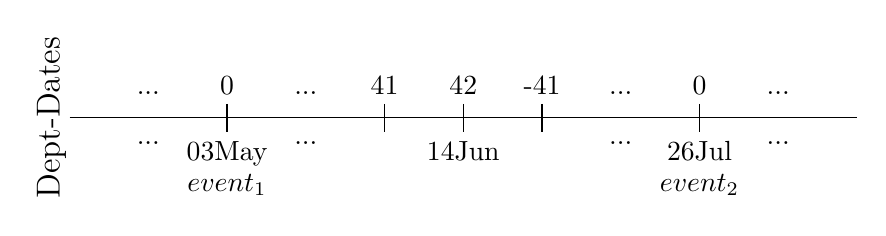
\begin{tikzpicture}
			\draw (0,0) -- (10,0);
			\foreach \x in {2, 4, 5, 6, 8}
			\draw (\x, 5pt) -- (\x, -5pt);
			\draw (2,0) node[below=5pt] {03May} node[above=5pt] {0};
			\draw (2,0) node[below=17pt] {$event_{1}$};
			\draw (4,0) node[above=5pt] {41};
			\draw (5,0) node[below=5pt] {14Jun} node[above=5pt] {42};
			\draw (6,0) node[above=5pt] {-41};
			\draw (8,0) node[below=5pt] {26Jul} node[above=5pt] {0};
			\draw (8,0) node[below=17pt] {$event_{2}$};
			\foreach \y in {1, 3, 7, 9}
			\draw (\y,0) node[below=5pt] {...} node[above=5pt] {...};
			\path (0,0) -- (10,0) node[rotate=90,midway,sloped,above=140] {\large Dept-Dates};
		\end{tikzpicture}
		\caption{The above demonstrates how event-times are defined relative to event-dates. First an example is given where a department is observed in one event. Second is an example of a multi-event department, where the mid-day between two events is the point at which event-times and event-days switch from referring to the prior event to refering to the latter.}
		\label{etime_diagram}
	\end{center}
\end{figure}

Afterwards, events are separated into ``high scrutiny" and ``low scrutiny" based on Trends data, which measures internet search volumes across 2011-2020 relative to George Floyd. If a deceased person's (or offending department) name was heavily searched after an event relative to its own pre-event mean, that death-event is considered to have generated ``high scrutiny". In this way, I strive to identify the most-watched departments and deceased people based on their associated events. \\

Following from the work of Grosjean, Masera \& Yousef (2023), this paper then collapses individual traffic stop observations to the dept-date level. From here, I generate outcome variables, by dept-date, for (1) black stop-share or the fraction of stops that are black, (2) the black search rate or the fraction of black stops that are searched, and (3) the black hit rate or the fraction of black searches that are successful. Each of these variables is used as an outcome in the following equations. Following from Becker (1957, 1993), particular attention is placed on the post-decision hit-rate outcome. \\

With this done, we arrive at the first estimation equation, whose resulting event-study graphs are shown in figures 4-6: \\

\begin{equation}
	\begin{split}
	Y^{o}_{d,t} = \gamma D^{[-270,-135)}_{d,t} + \sum_{\tau=105(15)30} \beta_{\tau}D^{[\tau,\tau+15)}_{d,t} + \\
		\delta D^{(135,270)}_{d,t} + \alpha_{d} + \theta_{t} + u_{d,t} 
	\end{split}
\end{equation}

Estimates taken for 15-day windows where $D^{a,b}_{d,t}=1$ if dept-date ($d,t$) stop observations occur between $a$ and $b$ days from an event, dropping the 15-day period prior to a shooting-event and using the 15-day window prior to that as a reference bin. Using 6 main outcomes with 6 corresponding volumetric outcomes, I am able to infer a lot about traffic stop behaviors. \\

The vector $Y^{o}$ consists of: (1) the black stop share, (2) the black search share, (3) the black hit share, (4) the black search \emph{rate}, (5) the black hit \emph{rate}, and (6) the black-hits to black-stops ratio. The volume-based outcomes are left to the appendix; (7) daily stop volume, (8) daily black stop volume, (9) daily search volume, (10) daily black search volume, (11) daily hit volume, and lastly (12) daily black hit volume. \\

From here, to analyze patterns across different scrutiny levels, a more robust equation is used, which considers all events but with a set of ``scrutiny" interaction bins which allow for closer examination of marginal effects of highly-publicized events separate from overall estimates: \\

\begin{equation} 
	\begin{split}
		Y^{o}_{d,t} = \gamma D^{[-270,-135)}_{d,t} + \sum_{\tau=-135(15)120} \beta_{\tau}D^{[\tau,\tau+15)}_{d,t} + \delta D^{[135,270]}_{d,t} + \\ 
		\zeta D_{d,t}*Sig_{d,t}^{[-270,-135)} + \sum_{\tau=-135(15)120} \Gamma_{\tau} D_{d,t}*Sig_{d,t}^{[\tau,\tau+15)} + \\ 
		\eta D_{d,t}*Sig_{d,t}^{[135,270]} + Sig_{d,t} + \alpha_{d} + \theta_{t} + u_{d,t}
	\end{split}
\end{equation}

Despite its appearance, this equation is fairly simple and nearly-identical to Equation 1, with two notable alterations: first, I add $Sig_{d,t}$ which is equal to 2 for treated groups if the nearest dept-date observation is considered highly scrutiny, 1 for low scrutiny, and 0 for control groups. Second, I interact this term with each of the $D_{d,t}$ dummy variables, which allows for a marginal-effects interpretation for highly-scrutinized events. \\

\begin{figure}
	\begin{center}
		\includegraphics[width=5.5in]{DiD_main_1.eps}
		\caption{The above t-statistics, which come from a DiD which corresponds to the pre/post-aggregation of Equation 2 - we see that the black share of stops has decreased, but otherwise outcomes are fairly stable following a death event. This would be consistent with reduced policing efforts on the front-end, but ``business as usual" practices once a stop has occurred.}
		\label{main_DiD_1}
	\end{center}
\end{figure}

\begin{figure}
	\begin{center}
		\includegraphics[width=5.5in]{DiDiD_main_1.eps}
		\caption{Splitting departments across scrutiny levels, we see that the decrease in black stop share is driven by the low-scrutiny events, with otherwise similar policing outcome patterns.}
		\label{main_DiDiD_1}
	\end{center}
\end{figure}

\begin{figure}
	\begin{center}
		\includegraphics[width=5.5in]{bstop_share.eps}
		\caption{As hinted at above, we see a decrease in the black stop share in the left column, and when allowing for different estimates for highly-scrutinized departments, we see a decrease in stop share only in the low-scrutiny departments.}
		\label{main_estudy_1}
	\end{center}
\end{figure}

\begin {figure}
	\begin{center}
		\includegraphics[width=5.5in]{bsearch_share.eps}
		\caption{The share of black searches remains fairly static, indicating that the ratio of black:non-black searches is stable following a death event.}
		\label{main_estudy_2}
	\end{center}
\end{figure}

\begin{figure}
	\begin{center}
		\includegraphics[width=5.5in]{bhit_share.eps}
		\caption{As with the search share, the hit rates are fairly static, perhaps noisy, but provide no evidence of a change in the black:non-black ratio of successful searches.}
		\label{main_estudy_3}
	\end{center}
\end{figure}

\begin {figure}
	\begin{center}
		\includegraphics[width=5.5in]{bsearch_rate.eps}
		\caption{Considering only stops of black drivers, we see that the rate at which they are searched remains stable. Once a stop has been made, it appears as though the rest of the encounter is fairly routine.}
		\label{main_estudy_4}
	\end{center}
\end{figure}

\begin {figure}
	\begin{center}
		\includegraphics[width=5.5in]{bhit_rate.eps}
		\caption{Considering only stops of black drivers which were then searched, we see that the success rate of a search, i.e. a hit, is unchanged.}
		\label{main_estudy_5}
	\end{center}
\end{figure}

\begin {figure}
	\begin{center}
		\includegraphics[width=5.5in]{bhit_bstop_ratio.eps}
		\caption{Finally, by removing the search information, we see that the nieve hit rate out of the full population of stops is stable following a death event.}
		\label{main_estudy_6}
	\end{center}
\end{figure}

%%%%%%%%%%%%%%%%%%%%%%%%%%%%%%%%%%%%%%%%%%%%%%%%%%%%%%%%%%%%%%%%%%%%%%%%%%%%%%%%%%%%%%%%%%%%%%%%%%%%

\section{Discussion:}

This article explores the relationship between traffic stops and fatal encounters at the hands of the police, a question that has gained a large amount of attention over recent years. Using a unique combination of datasets and a large set of observations spanning a full decade, I provide a highly-precise investigation of the dynamics in various traffic stop behaviors across time following a police-killing. \\

Theoretically, a lower stop share could be driven by either a decrease in the numerator (black stops), or the denominator (all stops). However, I have evidence that both of these values are decreasing, which in turn implies that the black stops are decreasing disproportionately to the non-black stops, relative to pre-event patterns. \\

Continuing from here, I find no evidence of post-stop changes in behaviors and outcomes. Black stopped drivers are being searched at similar ratios compared to non-black stopped drivers, and they are being found with contraband at similar ratios as well. The rate at which a black driver's stopped car is searched also remains unchanged, as does the hit rate following the searches. The overall ratio of black-driven cars which are stopped to the black-driven cars which are found with drugs also remains stable. \\

Taken together, these results imply that once a stop is made - what follows remains unchanged. This would be a consistent finding with the idea that police officers are decreasing their proactivity, a notion that is in-line with existant findings in the literature. \\

When splitting these events along scrutiny levels, I find that the overall decrease in the black-share of stops is being driven by low-scrutiny events. When being watched closely, it becomes more ``expensive" to lower policing efforts, there could be a subconscious desire to uphold the status quo and maintain consistent policing behaviors. \\

These results remain largely unchanged across my robustness checks where, (1) I drop the Tm1 period, (2) do not collapse to the dept-day level, (3) I use name-based scrutiny levels, (4) I keep the large statewide-departments. \\

In conclusion, I believe that policing efforts decrease following a death-event. I believe that this decrease is due to a combination of feeling unappreciated or even outright disliked, as well as a fear of becoming the next viral police interaction online. However, once a police officer commits to making a stop, I find no significant evidence of changes in what follows.  \\

%%%%%%%%%%%%%%%%%%%%%%%%%%%%%%%%%%%%%%%%%%%%%%%%%%%%%%%%%%%%%%%%%%%%%%%%%%%%%%%%%%%%%%%%%%%%%%%%%%%%

\section{References:}

Alpert, G. P., Smith, M. R., \& Dunham, R. G. (2004). Toward a better benchmark: Assessing the utility of not-at-fault traffic crash data in Racial Profiling Research. Justice Research and Policy, 6(1), 43–69. \url{https://doi.org/10.3818/jrp.6.1.2004.43} \\

ANG, D., \& TEBES, J. (2023). Civic responses to police violence. American Political Science Review, 118(2), 972–987. \url{https://doi.org/10.1017/s0003055423000515} \\

Antonovics, K., \& Knight, B. G. (2009). A new look at racial profiling: Evidence from the Boston Police Department. Review of Economics and Statistics, 91(1), 163–177. \url{https://doi.org/10.1162/rest.91.1.163} \\

Becker, G. S. (1971). The Economics of Discrimination. \url{https://doi.org/10.7208/chicago/9780226041049.001.0001} \\

Becker, G. S. (1993). Nobel lecture: The economic way of looking at behavior. Journal of Political Economy, 101(3), 385–409. \url{https://doi.org/10.1086/261880} \\

Cho, S., Gonçalves, F., \& Weisburst, E. (2023). The impact of fear on police behavior and public safety. SSRN Electronic Journal. \url{https://doi.org/10.2139/ssrn.4491235} \\

Deza, M., Lu, T., Maclean, J. C., \& Ortega, A. (2023). Behavioral health treatment and police officer safety. SSRN Electronic Journal. \url{https://doi.org/10.2139/ssrn.4491234} \\

Dube, A., Girardi, D., Jorda, O., \& Taylor, A. M. (2023). A local projections approach to difference-in-differences event studies. SSRN Electronic Journal. \url{https://doi.org/10.2139/ssrn.4433863} \\

Finch, B. K., Beck, A., Burghart, D. B., Johnson, R., Klinger, D., \& Thomas, K. (2019). “using crowd-sourced data to explore police-related-deaths in the United States (2000–2017): The case of fatal encounters.” Open Health Data, 6, 1. \url{https://doi.org/10.5334/ohd.30} \\

Goh, L. S. (2020). Going local: Do consent decrees and other forms of federal intervention in municipal police departments reduce police killings? Justice Quarterly, 37(5), 900–929. \url{https://doi.org/10.1080/07418825.2020.1733637} \\

Goncalves, F., \& Mello, S. (2021). A few bad apples? racial bias in policing. American Economic Review, 111(5), 1406–1441. \url{https://doi.org/10.1257/aer.20181607} \\

Grogger, J., \& Ridgeway, G. (2006). Testing for racial profiling in traffic stops from behind a veil of darkness. Journal of the American Statistical Association, 101(475), 878–887. \url{https://doi.org/10.1198/016214506000000168} \\

Grosjean, P., Masera, F., \& Yousaf, H. (2022). Inflammatory political campaigns and racial bias in policing. The Quarterly Journal of Economics, 138(1), 413–463. \url{https://doi.org/10.1093/qje/qjac037} \\

Hoekstra, M., \& Sloan, C. (2022). Does race matter for police use of force? evidence from 911 calls. American Economic Review, 112(3), 827–860. \url{https://doi.org/10.1257/aer.20201292} \\

Horrace, W. C., \& Rohlin, S. M. (2016). How dark is dark? bright lights, Big City, racial profiling. Review of Economics and Statistics, 98(2), 226–232. \url{https://doi.org/10.1162/rest\_a\_00543} \\

Kahn, K. B., \& Davies, P. G. (2017). What influences shooter bias? the effects of suspect race, neighborhood, and clothing on decisions to shoot. Journal of Social Issues, 73(4), 723–743. \url{https://doi.org/10.1111/josi.12245} \\

Kalinowski, J. J., Ross, M. B., \& Ross, S. L. (2023). Endogenous driving behavior in tests of racial profiling. Journal of Human Resources. \url{https://doi.org/10.3368/jhr.0822-12513r1} \\

Knowles, J., Persico, N., \& Todd, P. (2001). Racial bias in motor vehicle searches: Theory and evidence. Journal of Political Economy, 109(1), 203–229. \url{https://doi.org/10.1086/318603} \\

Mekawi, Y., \& Bresin, K. (2015). Is the evidence from racial bias shooting task studies a smoking gun? results from a meta-analysis. Journal of Experimental Social Psychology, 61, 120–130. \url{https://doi.org/10.1016/j.jesp.2015.08.002} \\

Miller, D. L. (2023). An introductory guide to event study models. Journal of Economic Perspectives, 37(2), 203–230. \url{https://doi.org/10.1257/jep.37.2.203} \\

Oramas Mora, D., Terrill, W., \& Foster, J. (2022). A Decade of Police use of Deadly Force Research (2011–2020). Homicide Studies, 27(1), 6–33. \url{https://doi.org/10.1177/10887679221123591} \\

Pierson, E., Corbett-Davies, S., \& Goel, S. (2018, March 31). Fast threshold tests for detecting discrimination. PMLR. \url{http://proceedings.mlr.press/v84/pierson18a.html} \\

Pierson, E., Simoiu, C., Overgoor, J., Corbett-Davies, S., Jenson, D., Shoemaker, A., Ramachandran, V., Barghouty, P., Phillips, C., Shroff, R., \& Goel, S. (2020). A large-scale analysis of racial disparities in police stops across the United States. Nature Human Behaviour, 4(7), 736–745. \url{https://doi.org/10.1038/s41562-020-0858-1} \\

Powell, Z. A. (2022). De-policing, police stops, and crime. Policing: A Journal of Policy and Practice, 17. \url{https://doi.org/10.1093/police/paac070} \\

Renner, M. L. (2018). Using multiple flawed measures to construct valid and reliable rates of homicide by police. Homicide Studies, 23(1), 20–40. \url{https://doi.org/10.1177/1088767918786756} \\

Simoiu, C., Corbett-Davies, S., \& Goel, S. (2017). The problem of infra-marginality in outcome tests for discrimination. The Annals of Applied Statistics, 11(3). \url{https://doi.org/10.1214/17-aoas1058} \\

Voigt, R., Camp, N. P., Prabhakaran, V., Hamilton, W. L., Hetey, R. C., Griffiths, C. M., Jurgens, D., Jurafsky, D., \& Eberhardt, J. L. (2017). Language from police body camera footage shows racial disparities in officer respect. Proceedings of the National Academy of Sciences, 114(25), 6521–6526. \url{https://doi.org/10.1073/pnas.1702413114} \\


%%%%%%%%%%%%%%%%%%%%%%%%%%%%%%%%%%%%%%%%%%%%%%%%%%%%%%%%%%%%%%%%%%%%%%%%%%%%%%%%%%%%%%%%%%%%%%%%%%%%

\section{Appendix:}

%%% EQUATION 1 APPENDIX FIGURES %%%
\begin{figure}
	\begin{center}
		\includegraphics[width=5.5in]{DiD_main_2.eps}
		\caption{Turning to volume-based outcomes, we see that the stop and search volumes are likely decreasing following a fatal event. Taken together with the share outcomes from above, all stops may be decreasing, but black outcomes are decreasing disproportionately so relative to their pre-event ratios.}
		\label{main_DiD_2}
	\end{center}
\end{figure}

\begin{figure}
	\begin{center}
		\includegraphics[width=5.5in]{DiDiD_main_2.eps}
		\caption{Allowing for different effects in department scrutiny levels, we see that once again the decreases in volume are occurring differently when scrutiny levels are low vs high.}
		\label{main_DiDiD_2}
	\end{center}
\end{figure}

\begin{figure}
	\begin{center}
		\includegraphics[width=5.5in]{n_stops.eps}
		\caption{As discussed, we have suggestive evidence of a decrease in stop volume, but this is primarily being driven by low scrutiny events.}
		\label{main_estudy_7}
	\end{center}
\end{figure}

\begin{figure}
	\begin{center}
		\includegraphics[width=5.5in]{n_bstops.eps}
		\caption{As with all-stops, the black stops are decreasing somewhat, and this is being driven by the low-scrutiny events.}
		\label{main_estudy_8}
	\end{center}
\end{figure}

\begin{figure}
	\begin{center}
		\includegraphics[width=5.5in]{n_searches.eps}
		\caption{As before, the volume of searches decreases, primarily through low scrutiny events.}
		\label{main_estudy_9}
	\end{center}
\end{figure}

\begin{figure}
	\begin{center}
		\includegraphics[width=5.5in]{n_bsearches.eps}
		\caption{With black searches, we see the same pattern as in all-searches. Decreases are not significant, but they appear to differ along scrutiny levels.}
		\label{main_estudy_10}
	\end{center}
\end{figure}

\begin{figure}
	\begin{center}
		\includegraphics[width=5.5in]{n_hits.eps}
		\caption{The volume of successful searches appears to be almost entirely unaffected following a death event, regardless of scrutiny.}
		\label{main_estudy_11}
	\end{center}
\end{figure}

\begin{figure}
	\begin{center}
		\includegraphics[width=5.5in]{n_bhits.eps}
		\caption{As with all-hits, the black hit volume appears to be unaffected by events regardless of scrutiny levels.}
		\label{main_estudy_12}
	\end{center}
\end{figure}

If you are reading this - thank you! \\

\end{document}
